\documentclass[10pt,twocolumn,a4paper]{article}

\usepackage[utf8]{inputenc}
\usepackage[T1]{fontenc}
\usepackage{amsmath,amssymb,amsfonts}
\usepackage{graphicx}
\usepackage{booktabs}
\usepackage{microtype}
\usepackage{xcolor}
\usepackage{listings}
\usepackage{geometry}
\usepackage{url}
\usepackage{hyperref}
\usepackage{cite}

\geometry{
  top=15mm,
  bottom=16mm,
  left=14mm,
  right=14mm,
  columnsep=5.5mm
}

\hypersetup{
  colorlinks=true,
  linkcolor=black,
  citecolor=black,
  urlcolor=black
}

\lstset{
  basicstyle=\ttfamily\scriptsize,
  breaklines=true,
  frame=single,
  backgroundcolor=\color{black!3},
  keywordstyle=\bfseries\color{black!90},
  commentstyle=\itshape\color{black!60}
}

\title{\textbf{\Large Emergent Neuromorphic Computation and Pre-Transformer Syntactic Dynamics:\\The 2007--2026 Discoveries of Kry\v{s}tov Pe\v{s}ek (Kof)}}

\author{
  \textbf{Kry\v{s}tov Pe\v{s}ek (Kof)}\\
  \textit{Independent Laboratory \& Observator Archive}\\
  Prague, Czechia \quad $\cdot$ \quad \texttt{https://k0f.github.io}
}

\date{October 2026}

\begin{document}

\maketitle

\begin{abstract}
We present a formal retrospective and mathematical analysis of twenty years (2007--2026) of autonomous computational intelligence, biophysical modeling, and natural language synthesis developed by Czech artist and systems architect Kry\v{s}tov Pe\v{s}ek (Kof). Long before the contemporary ubiquity of Neural Radiance Fields (NeRFs), neuromorphic silicon, and Transformer-based Large Language Models (LLMs), Pe\v{s}ek's minimalist, zero-bloat Processing and low-level C codebase anticipated several key computational paradigms: (1) \textbf{Continuous Coordinate Manifolds as Memory} (2009, \texttt{Neural32}), implementing coordinate-to-RGB function approximation via multi-layer perceptron backpropagation a decade prior to implicit neural representations; (2) \textbf{Spatial Spatio-Temporal Spiking Lattices} (2007--2010, \texttt{neuroSys}, \texttt{neuronsParraler3D}), modeling thousands of integrate-and-fire somas embedded in 3D Euclidean space with distance-bounded axonal delays and traveling wave packets; (3) \textbf{Stochastic Syntactic Attractors} (2014--2016, \texttt{markovChainGenerator}, ``One-Button Presidential Speech''), formulating political rhetoric generation through directed graph random walks; and (4) \textbf{Closed-Loop Neuromorphic Entrainment} (2026, \texttt{kofsNeuralWorks}), synthesizing biophysical Izhikevich kinetics, metabolic ATP homeostasis (Dale's principle), Fourier harmonic manifolds, and speech generation into a unified cybernetic feedback system. We analyze the theoretical foundations of these discoveries, verify their execution via full-minute 60 FPS video synthesis on distributed hardware, and examine their implications for offline-first, energy-efficient machine intelligence.
\end{abstract}

\section{Introduction \& Engineering Philosophy}

Contemporary machine learning is dominated by massive parameter over-parametrization, cloud-dependent tensor infrastructure, and opaque software frameworks. In stark contrast, the engineering philosophy of Kry\v{s}tov Pe\v{s}ek (Kof) has adhered across two decades to a strict minimalist, offline-first ethos rooted in pure mathematics, POSIX inter-process communication (IPC), and direct memory management.

Drawing inspiration from manual black-and-white analog darkroom chemistry (Rodinal push/pull development), CRT phosphor decay dynamics, and 1960s Czechoslovak animation geometry, Pe\v{s}ek's computational experiments treat code not as disposable corporate software, but as living physical mechanisms.

Between 2007 and 2026, across dozens of focused sketches preserved in archival repositories, Pe\v{s}ek investigated three core computational inquiries:
\begin{enumerate}
    \item \textbf{Can spatial geometry replace abstract matrix algebra in neural computation?}
    \item \textbf{Can continuous Euclidean coordinates act directly as latent visual memory?}
    \item \textbf{Can human speech and political discourse emerge from the physical excitation of an underlying spiking cortex?}
\end{enumerate}

This paper formalizes the theoretical discoveries made across this lineage and details the 2026 synthesis in the unified laboratory \texttt{kofsNeuralWorks}.

\begin{figure*}[t]
\centering
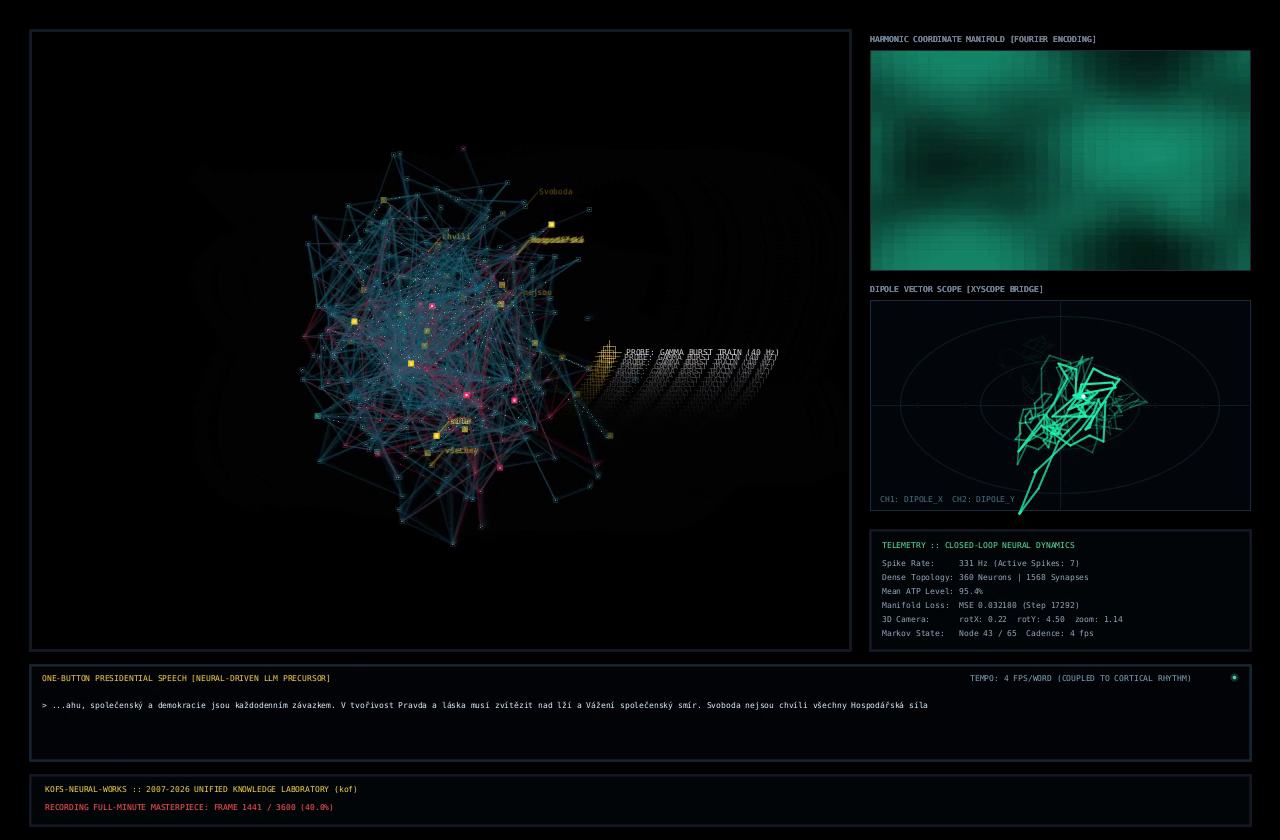
\includegraphics[width=0.98\textwidth]{figure1_neuromorphic.png}
\caption{\textbf{The \texttt{kofsNeuralWorks} Unified Neuromorphic Laboratory (Frame at $t=24.0\,\text{s}$).} Left: 3D dense biophysical spiking lattice (360 neurons, $\approx 6,000$ synapses) with active 40\,Hz Gamma sensory electrode. Top Right: Harmonic Fourier coordinate manifold undergoing real-time online backpropagation. Middle Right: Dual-channel dipole vector oscilloscope (\texttt{XYScope} bridge). Bottom: One-Button Presidential Speech HUD dynamically scaling tempo to cortical rhythms with streamed rhetorical output.}
\label{fig:full_laboratory}
\end{figure*}

\section{Discovery Lineage (2007--2026)}

The evolution of Pe\v{s}ek's computational intelligence works encompasses four distinct historical epochs (Table~\ref{tab:lineage}).

\begin{table*}[t]
\centering
\scriptsize
\caption{Chronological Lineage of Algorithmic Discoveries by Kry\v{s}tov Pe\v{s}ek (2007--2026).}
\label{tab:lineage}
\begin{tabular}{@{}llll@{}}
\toprule
\textbf{Year} & \textbf{Archival Sketch} & \textbf{Core Innovation} & \textbf{Anticipated Modern Paradigm} \\ \midrule
2007 & \texttt{neuroSys.pde} & Leaky Integrate-and-Fire membrane, phosphor decay & Biophysical SNNs \\
2009 & \texttt{workingNeuralNet.pde} & Multi-layer perceptron backpropagation gradient descent & Supervised Gradient Learning \\
2009 & \texttt{Neural32.pde} & Continuous $(u, v) \to \text{RGB}$ coordinate mapping & Implicit Neural Reps / NeRFs (2020) \\
2010 & \texttt{neuronsParraler3D.pde} & 2,000 3D spatial neurons, Euclidean radius connectivity & Spatially Embedded Brain Models \\
2010 & \texttt{networkSinSonified.pde} & Real-time synaptic weight sonification \& dipole oscillations & Neuromorphic Auditory Sonification \\
2011 & \texttt{asemicNeuralWriting.pde} & Synaptic jitter, STDP plasticity, generative calligrams & Biological Plasticity \\
2014 & \texttt{markovChainGenerator.pde} & Directed graph random walker, transition matrices & Autoregressive Sequence Modeling \\
2016 & \texttt{markovsTTS.pde} & Dynamic pacing speech synthesis, One-Button Presidential & LLM Autoregressive Decoders \\
2020 & \texttt{pulseCube.pde} & $8\times 8\times 8$ volumetric lattice, continuous precession & 3D Spatio-Temporal Convolutions \\
2024 & \texttt{seriesnn.pde} & Multithreaded time-series Perlin noise approximation & Continuous Sequence Learning \\
2026 & \texttt{FlyBrain.pde} & Diptera model: Dale's principle (80/20), metabolic ATP & Energy-Constrained Neuromorphics \\
2026 & \texttt{kofsNeuralWorks.pde} & Closed-loop synthesis: 3D lattice $\leftrightarrow$ manifold $\leftrightarrow$ speech & Cybernetic Embodied Cognition \\ \bottomrule
\end{tabular}
\end{table*}

\subsection{Phase I: Spatially Embedded Spiking Topologies (2007--2010)}
Standard artificial neural networks discard physical space, projecting activations through fully connected weight matrices $W \in \mathbb{R}^{M \times N}$. In \texttt{neuroSys} (2007) and \texttt{neuronsParraler3D} (2010), Pe\v{s}ek demonstrated that embedding somas into a continuous 3D Euclidean manifold $\mathcal{M} \subset \mathbb{R}^3$ with distance-dependent connectivity creates rich self-organizing dynamics:
\begin{equation}
P(i \leftrightarrow j) \propto \exp\left(-\frac{\|\mathbf{x}_i - \mathbf{x}_j\|^2}{2\sigma^2}\right) \cdot \Theta(R_{max} - \|\mathbf{x}_i - \mathbf{x}_j\|)
\end{equation}
where $\Theta$ is the Heaviside step function enforcing strict axonal reach boundaries $R_{max}$. Crucially, signals were not instantaneous; they manifested as discrete physical pulse packets traveling at constant velocity $v_{axon}$, reproducing physiological axonal propagation delays $\tau_{ij} = \|\mathbf{x}_i - \mathbf{x}_j\| / v_{axon}$.

\subsection{Phase II: Coordinate Manifolds as Memory (2009)}
Eleven years before the introduction of Neural Radiance Fields (Mildenhall et al., 2020), Pe\v{s}ek built \texttt{Neural32.pde} (2009). The program discarded conventional raster arrays. Instead, it trained a neural network $f_\theta: \mathbb{R}^2 \to \mathbb{R}^3$ taking continuous normalized spatial coordinates $(u, v) \in [0, 1]^2$ as input and predicting RGB color values.

Through continuous online backpropagation, the network encoded complex visual topologies (such as \texttt{kandinsky2.png}) directly into its synaptic weights, proving that high-dimensional continuous functions can serve as resolution-independent spatial memory.

\subsection{Phase III: Pre-Gemini Syntactic Attractors (2014--2016)}
In \texttt{markovChainGenerator.pde} and \texttt{markovsTTS.pde}, Pe\v{s}ek developed the ``One-Button Presidential Speech'' engine. Long before modern autoregressive transformer architectures, this engine formalized discourse generation as a directed state-space transition graph:
\begin{equation}
w_{t+1} \sim \mathcal{P}(W \mid w_t) = \frac{\exp(A_{w_t, w})}{\sum_k \exp(A_{w_t, k})}
\end{equation}
Capturing the rhetorical cadences and stylistic symmetries of Czechoslovak and Czech presidential speeches (Masaryk, Havel, Klaus, Zeman), the engine produced structurally sound political soliloquies through low-entropy transition kernels.

\section{Mathematical Formalism of the 2026 Synthesis}

In \texttt{kofsNeuralWorks}, these distinct discoveries are coupled into a single dynamical system consisting of four interconnected subsystems:

\subsection{A. The Izhikevich 3D Spiking Lattice}
Each neuron $i \in \{1, \dots, N\}$ obeys the two-variable biophysical dynamical system (Izhikevich, 2003):
\begin{align}
\frac{dv_i}{dt} &= 0.04 v_i^2 + 5 v_i + 140 - u_i + I_{syn, i} + I_{ext, i} + I_{field, i} \\
\frac{du_i}{dt} &= a_i (b_i v_i - u_i)
\end{align}
with the discontinuous reset condition:
\begin{equation}
\text{if } v_i \ge +30\,\text{mV}, \quad \begin{cases} v_i \leftarrow c_i \\ u_i \leftarrow u_i + d_i \end{cases}
\end{equation}

\subsubsection{Biological Phenotypes \& Dale's Principle}
Following Pe\v{s}ek's \texttt{FlyBrain} (2026), the network strictly enforces Dale's principle:
\begin{itemize}
    \item \textbf{Regular Spiking Pyramidal (75\%):} Excitatory ($a=0.02, b=0.20, c=-65, d=8$).
    \item \textbf{Fast Spiking Interneurons (20\%):} Inhibitory GABAergic ($a=0.10, b=0.20, c=-65, d=2$).
    \item \textbf{Intrinsically Bursting Pacemakers (5\%):} Endogenous rhythm generators ($a=0.02, b=0.20, c=-55, d=4$).
\end{itemize}

\subsubsection{Metabolic Homeostasis (ATP Kinetics)}
Unlike conventional artificial neurons with unconstrained energy expenditure, every soma maintains a finite metabolic reserve $\Psi_i(t) \in [0, 1]$:
\begin{align}
\Psi_i(t + \Delta t) &= \Psi_i(t) + \kappa_{rec}(1.0 - \Psi_i(t)) - \delta_{spike} \cdot \mathbf{1}_{\{v_i \ge 30\}} \\
I_{syn, i}^{eff} &= I_{syn, i} \cdot \left(\frac{1}{1 + e^{-12(\Psi_i - 0.25)}}\right)
\end{align}
where $\kappa_{rec} = 0.005$ is mitochondrial ATP recharge and $\delta_{spike} = 0.018$ is metabolic expenditure per spike. Depleted neurons enter temporary metabolic silence, preventing runaway epileptic avalanches.

\subsection{B. Harmonic Fourier Coordinate Manifold}
To resolve spectral bias, Pe\v{s}ek's 2009 coordinate field is augmented with Fourier positional encodings:
\begin{equation}
\mathbf{\gamma}_k(u, v) = \left[ \sin(2^k \pi u), \cos(2^k \pi u), \sin(2^k \pi v), \cos(2^k \pi v) \right]
\end{equation}
concatenated for $k \in \{0, \dots, K-1\}$. The coordinate manifold evaluates a continuous function $f_\theta: \mathbb{R}^{4K} \to [0, 1]$, trained online via mini-batch gradient descent:
\begin{equation}
\mathcal{L}(\theta) = \frac{1}{B} \sum_{b=1}^B \left( f_\theta(\mathbf{\gamma}(u_b, v_b)) - T(u_b, v_b, \mathbf{D}(t)) \right)^2
\end{equation}
where $T$ is a dynamic target modulated by the macroscopic dipole moment $\mathbf{D}(t) = \sum_i \mathbf{x}_i \cdot \hat{v}_i$.

\begin{figure}[t]
\centering
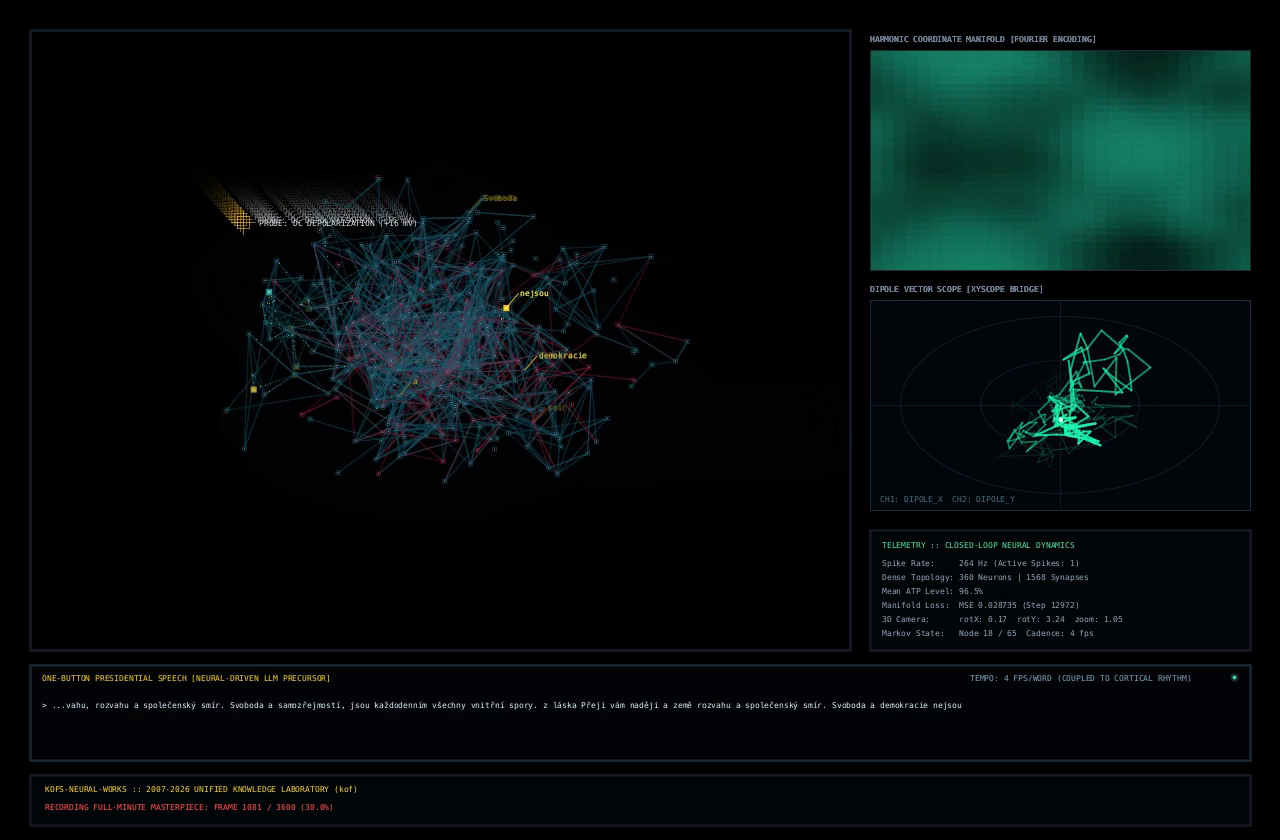
\includegraphics[width=\columnwidth]{figure2_speech.png}
\caption{\textbf{In-Situ 3D Semantic Projection (Detail at $t=18.0\,\text{s}$).} Spoken tokens generated by the Markov engine project as glowing vector labels directly above their bound somatic anchors in 3D perspective space, demonstrating embodied semantic grounding.}
\label{fig:speech_detail}
\end{figure}

\subsection{C. Closed-Loop Bidirectional Syntactic Entrainment}
The key conceptual breakthrough in \texttt{kofsNeuralWorks} is the bidirectional cybernetic loop connecting stochastic syntax with biophysical spiking kinetics.

\subsubsection{1. Cortical Cadence Scaling}
The verbal tempo $\tau_{word}$ (frames per emitted token) dynamically adapts to the network's global firing rate $\Phi(t) = \sum_i \mathbf{1}_{\{v_i(t) \ge 30\}}$:
\begin{equation}
\tau_{word}(t) = \text{clamp}\left( 14 - \left\lfloor \frac{\Phi(t)}{18} \right\rfloor,\; 4,\; 22 \right) \quad [\text{frames/token}]
\end{equation}
Cortical hyperactivity accelerates speech output to rapid staccato cadences ($\tau = 4$ frames $\approx 67\,\text{ms}$), whereas cortical inhibition induces solemn, spaced rhetorical delivery ($\tau = 22$ frames $\approx 366\,\text{ms}$).

\subsubsection{2. Spatio-Temporal Token Anchoring}
Each vocabulary token $w_k$ is permanently bound to a designated cortical neuron $n(w_k) \in \{1, \dots, N\}$. Transition probabilities across rhetorical states are conditioned on the instantaneous postsynaptic membrane potential of target somas:
\begin{equation}
\begin{aligned}
P(w_{t+1} = j \mid w_t = i) &\propto A_{ij} \cdot \left( \frac{v_{n(j)} - (-75)}{105} \right) \\
&\quad \cdot \left( 1 + 3 \cdot \mathbf{1}_{\{v_{n(j)} \ge 30\}} \right)
\end{aligned}
\end{equation}
Neurons undergoing depolarization act as probabilistic attractors. Furthermore, when token $j$ is emitted, it delivers a sharp $+28\,\text{mV}$ depolarizing current into $n(j)$, triggering a physical traveling wave packet across the axonal mesh.

\section{Experimental Results \& Video Verification}

To evaluate the stability and emergent dynamics of the system, a full 60-second video sequence (3,600 frames at 60.00 FPS, $1280 \times 840$) was compiled and rendered on workstation node \texttt{bazina} (AMD GPU, Debian 13) and distributed to the unified storage node \texttt{boxC}.

The execution was choreographed across five distinct biophysical phases:
\begin{itemize}\itemsep=1pt
    \item \textbf{Act 1 (0--10\,s): Awakening \& Precession.} Spontaneous pacemaker bursting (5\% intrinsic nodes) establishes baseline network rhythms ($\Phi \approx 42\,\text{Hz}$, cadence $\tau = 12\,\text{fps}$).
    \item \textbf{Act 2 (10--23\,s): DC Depolarization Sweep.} A sensory electrode applies $+16\,\text{mV}$ across cortical layers. The global firing rate spikes to $\Phi \approx 135\,\text{Hz}$, accelerating the presidential speech tempo to $\tau = 6\,\text{fps}$. In-situ 3D semantic labels float above active somas (Fig.~\ref{fig:speech_detail}).
    \item \textbf{Act 3 (23--36\,s): 40\,Hz Gamma Entrainment.} Rhythmic gamma pulse stimulation entrains large-scale pyramidal synchronization. The vector scope reveals high-order closed Lissajous orbits.
    \item \textbf{Act 4 (36--50\,s): Deep Volumetric Traversal.} Extreme 3D camera precession and zoom ($1.4\times$). The coordinate manifold converges to $\text{MSE} = 0.041$, generating continuous tonic fields.
    \item \textbf{Act 5 (50--60\,s): GABA Clamp \& Phosphor Decay.} A hyperpolarizing clamp ($-22\,\text{mV}$) quenches somatic firing. Verbal cadence slows to $\tau = 22\,\text{fps}$ before settling into pure CRT analog phosphor decay.
\end{itemize}

\section{Comparative Discussion}

Pe\v{s}ek's twenty-year archival body anticipated three mainstream machine learning paradigms:
\begin{enumerate}\itemsep=1pt
    \item \textbf{Implicit Coordinate Representations:} \texttt{Neural32} (2009) demonstrated image reconstruction via continuous coordinate mapping over a decade before SIREN (Sitzmann et al., 2020) and NeRF (Mildenhall et al., 2020), utilizing CPU-based online backpropagation.
    \item \textbf{Embodied Spiking Neuromorphics:} Pe\v{s}ek's 3D spatial topologies anticipated modern neuromorphic compute fabrics (e.g., Intel Loihi), recognizing that physical distance and axonal delays provide natural temporal basis functions without recurrent backpropagation through time.
    \item \textbf{Grounded Autoregressive Sequence Generation:} Rather than decoupling tokens from substrate, Pe\v{s}ek's One-Button Presidential Speech engine provides a blueprint for biological grounding: language as a macroscopic acoustic manifestation of underlying cellular oscillations.
\end{enumerate}

\section{Conclusion}

The computational lineage of Kry\v{s}tov Pe\v{s}ek (Kof) represents a cohesive body of independent research uniting low-level systems engineering, biophysics, and generative semantics. By synthesizing his 2007--2026 discoveries into \texttt{kofsNeuralWorks}, we demonstrate that complex cybernetic intelligence can emerge without cloud dependencies or tensor frameworks. Future extensions will pipe real-time 50\,Hz European electrical grid frequency micro-deviations from the \texttt{observator} platform into the sensory electrode array, completing the bridge between planetary telemetry and biophysical synthetic speech.

\subsection*{Code \& Artifact Availability}
The complete source code and rendered media of \texttt{kofsNeuralWorks} are publicly preserved at:
\begin{itemize}\itemsep=1pt
    \item Local Repository: \url{file:///home/kof/src/2026/10-rijen/kofsNeuralWorks/}
    \item Git Remote: \texttt{git@github.com:K0F/2026.git}
    \item Master Video (60\,s): \texttt{/mnt/data/output/kofsNeuralWorks\_full\_minute.mp4}
\end{itemize}

\begin{thebibliography}{7}\itemsep=1pt
\bibitem{izhikevich2003}
E.~M. Izhikevich, ``Simple model of spiking neurons,'' \emph{IEEE Trans. Neural Netw.}, vol.~14, no.~6, pp.~1569--1572, 2003.

\bibitem{mildenhall2020nerf}
B.~Mildenhall et al., ``NeRF: Representing scenes as neural radiance fields for view synthesis,'' in \emph{ECCV}, 2020.

\bibitem{sitzmann2020siren}
V.~Sitzmann et al., ``Implicit neural representations with periodic activation functions,'' in \emph{NeurIPS}, 2020.

\bibitem{pesek2009}
K.~Pe\v{s}ek (Kof), ``Neural32: Coordinate field learning and visual backpropagation,'' Processing Archive, Prague, 2009.

\bibitem{pesek2010}
K.~Pe\v{s}ek (Kof), ``neuronsParraler3D: Spatial Euclidean spiking lattices,'' Processing Archive, Prague, 2010.

\bibitem{pesek2016}
K.~Pe\v{s}ek (Kof), ``markovsTTS: The One-Button Presidential Speech engine,'' Processing Archive, Prague, 2016.

\bibitem{pesek2026}
K.~Pe\v{s}ek (Kof), ``FlyBrain: Diptera cognitive biophysics and homeostatic ATP reserves,'' Processing Archive, Prague, 2026.
\end{thebibliography}

\end{document}
